\chapter{\singlecelltitle}
\label{chap:heterogeneity}
\glsresetall
\clearpage

\section{Abstract}
\par\textit{Motivation ---} Intratumoral copy number heterogeneity of \gls{ecDNA} in single cells of a tumor is widely believed to contribute to tumor evolution and drug resistance. The capacity to count ecDNA in a large number of single cells would enable the observation of this heterogeneity in sequential tumor biopsies, revealing the population dynamics of ecDNA under therapeutic selection. Numerous algorithms have been developed to estimate genomic copy number from single-cell sequencing data. However, none are designed to quantify ecDNA copy number from single-cell profiles of accessible chromatin (scATAC-seq).
\par\textit{Results ---} To estimate the copy number of a known ecDNA sequence from scATAC-seq data, we compare sequencing read coverage at the ecDNA locus to that elsewhere in the genome. \gls{ecDNA} copy number estimated by this approach strongly correlates to transcriptional measures of ecDNA activity. We apply our method to a dataset of multiome single cell ATAC + Gene Expression (scRNA+ATAC-seq) data from the primary human tumor (HT) and patient-derived xenograft (PDX) of a p53-mutant, SHH subgroup medulloblastoma (MB), and show that \gls{ecDNA+} cells were strongly selected during PDX model establishment. We orthogonally validate our model by estimating ecDNA copy number in the same tumor using automated image analysis on FISH imaging of interphase nuclei stained for ecDNA.
\par\textit{Availability and implementation ---} A software implementation of our approach is available at \url{ https://github.com/auberginekenobi/ecdna-quant}.

\section{Introduction}
\par Intratumoral copy number heterogeneity of extrachromosomal circular DNA (\gls{ecDNA}) in single cells of a tumor is widely believed to contribute to tumor evolution, drug resistance, and poor patient outcomes \cite{bafna_2022}. In the previous chapter, we detected circular ecDNA by assembling cyclic sequences in short-read \gls{wgs} of bulk patient tissue, enabling us to survey a large retrospective cohort of patient data. However, assembly of bulk \gls{wgs} cannot distinguish variation of ecDNA sequence, copy number, and and gene expression between tumor cells, limiting our capacity to measure intratumoral heterogeneity within a given tumor sample. Therefore, to understand the population dynamics of an ecDNA+ tumor, it is necessary to employ emerging methods to examine ecDNA at single-cell resolution. 
\par To address this challenge, we have applied four orthogonal technologies to the \gls{pdx} MB model tumor RCMB56-pdx. We apply \gls{ogm} and CRISPR-CATCH \cite{crispr-catch} to reconstruct high-confidence sequence assemblies of 2 ecDNA lineages originating from distinct portions of the reference human genome, and show that both sequences are conserved in the corresponding patient tumor RCMB56-ht. Next, we analyze FISH microscopy and single-cell sequencing data to estimate ecDNA copy number amplification at single-cell resolution, and show that a clonal expansion of ecDNA+ cells occurred during the engraftment interim between RCMB56-ht and RCMB56-pdx. We anticipate that similar approaches may shed light on clonal dynamics of ecDNA+ cell populations under other selective pressures such as conventional or targeted therapy.

\section{Results}
\subsection{Linear and circular extrachromosomal amplifications co-exist in the RCMB56 patient tumor and PDX model.}
We have previously described a SHH MB primary tumor with heterozygous somatic \textit{TP53} mutation (\acrshort{rcmb56-ht}) \cite{rusert_2020}, which we have established as a PDX model (\acrshort{rcmb56-pdx}). Analysis of WGS from \acrshort{rcmb56-ht} predicted two distinct amplifications, a circular ecDNA of length 3.2Mbp comprising three regions of chr1 (amp1, Fig. \ref{subfig:rcmb56-ar-1}), and a complex, possibly chromothriptic, 4.5Mbp amplicon comprising 21 segments of chr7 and chr17, with ends mapping to pericentromeric and peritelomeric regions (amp2, Fig. \ref{subfig:rcmb56-ar-2}). Analysis of \gls{wgs} from \acrshort{rcmb56-pdx} confirmed that both focal amplifications were unchanged as compared to the original primary human tumor. To assemble high-confidence sequences for the two amplicons, we performed optical genome mapping (OGM, Bionano Genomics) of \gls{uhmw dna} from \acrshort{rcmb56-pdx}. Assembly from deep \gls{wgs} and \gls{ogm} validated the circular amp1 composed of three DNA segments from chr1 (Fig. \ref{subfig:rcmb56-ar-1}). This analysis also validated the contiguous chromothriptic amplification comprising 21 segments of chr7 and chr17; however, a circular structure could not be conclusively established from \gls{ogm} and \gls{wgs} data (Fig. \ref{subfig:rcmb56-ar-2}). Copy number of amp1 and amp2 was estimated from WGS data at 20 and 10 in \acrshort{rcmb56-ht}, and 30 and 25 in \acrshort{rcmb56-pdx} (Suppl. Figs. 5-6 of \cite{Chapman}). 

\begin{figure}[!h]
    \centering
    \begin{subfigure}{0.49\textwidth}
        \centering
        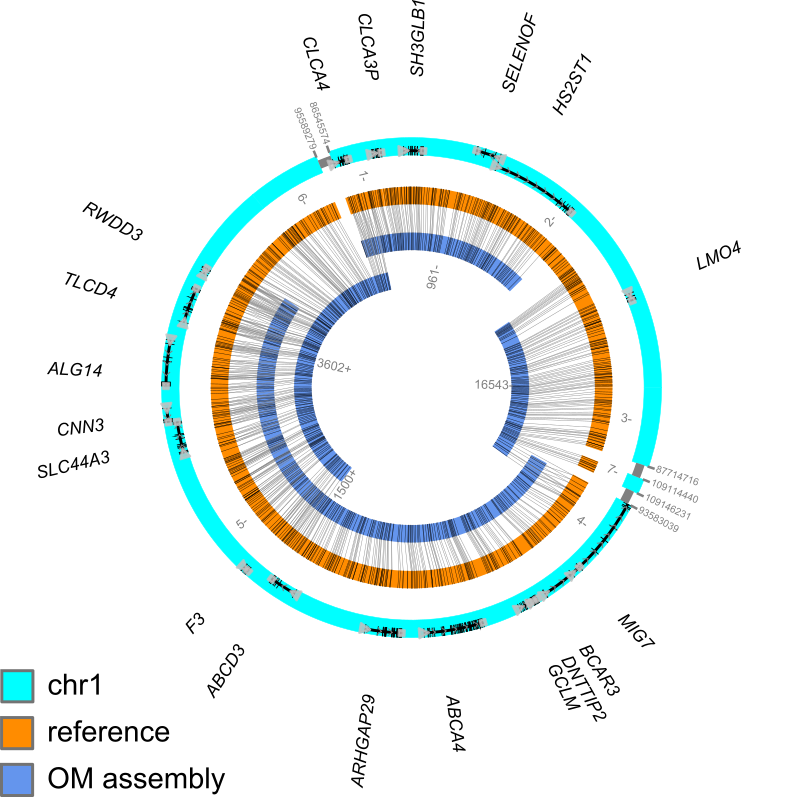
\includegraphics{RCMB56-amp1-AR}
        \caption{}
        \label{subfig:rcmb56-ar-1}
    \end{subfigure}
    \begin{subfigure}{0.49\textwidth}
        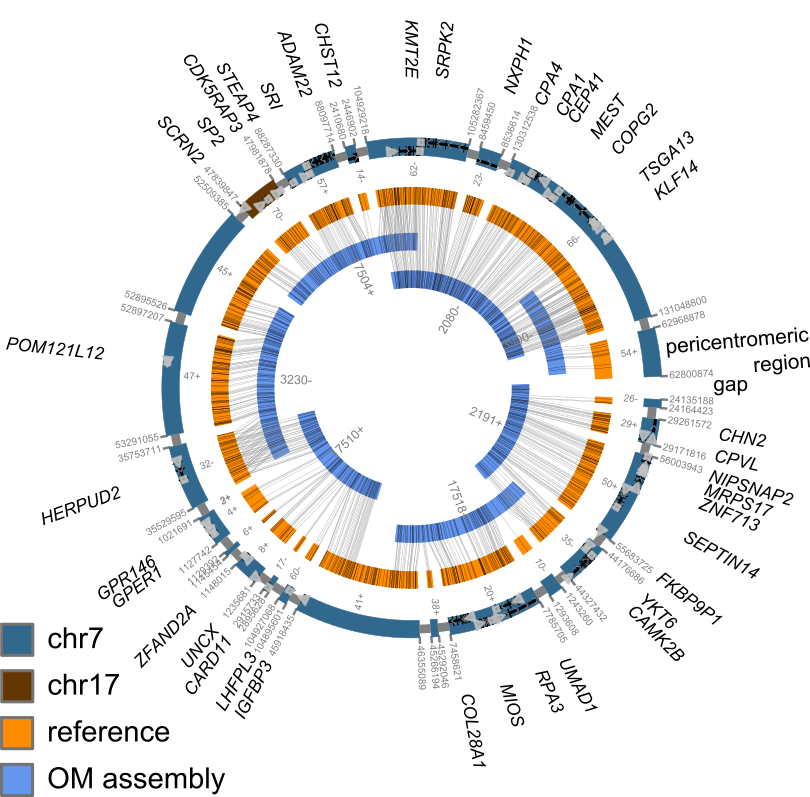
\includegraphics{RCMB56-amp2-AR}
        \caption{}
        \label{subfig:rcmb56-ar-2}
    \end{subfigure}
    \caption[Sequence assemblies of extrachromosomal amplifications in RCMB56.]{\textbf{Sequence assemblies of extrachromosomal amplifications in RCMB56.} (\textbf{a}) RCMB56 amp1 is a circular amplification composed of 3 segments of chr1p. (\textbf{b}) RCMB56 amp2 is a noncircular assembly composed of 21 segments of chr7 and chr17. Ends of the assembly map to pericentromeric (pictured, supported by \gls{wgs} and \gls{ogm} data) and peritelomeric (not pictured, supported by \gls{wgs} data only) regions of chr7. Sequences were assembled from \gls{wgs} aligned to the hg38 reference genome and scaffolded by \gls{ogm} data \cite{Kim_2020}.}
    \label{fig:rcmb56-ar}
\end{figure}

To further validate the sequence assemblies of amp1 and amp2, we used a recent method for targeted profiling of ecDNA, CRISPR-CATCH \cite{crispr-catch}. As expected, cutting amp1 in UHMW DNA from RCMB56-pdx produced a single fraction of DNA with the predicted length of ecDNA amp1. Moreover, short read sequencing maps this DNA to the amp1 sequence identified from bulk sequencing, confirming its circular structure  (Fig. \ref{fig:cc}a-b). 

Cutting amp2 produced 2 distinct fractions of DNA with lengths substantially shorter than amp2, which mapped to mutually exclusive segments of the amp2 assembly. Not cutting amp2 produced a single fraction with the predicted length of amp2 and mapping to the amp2 sequence (Fig. \ref{fig:cc}c-d). Both observations are consistent with the linear sequence assembly shown in Fig. \ref{subfig:rcmb56-ar-1}, and inconsistent with a hypothetical sequence linking the two ends of the amp2 assembly.

\begin{figure}[p]
    \centering
    \begin{subfigure}{0.49\textwidth}
        \centering
        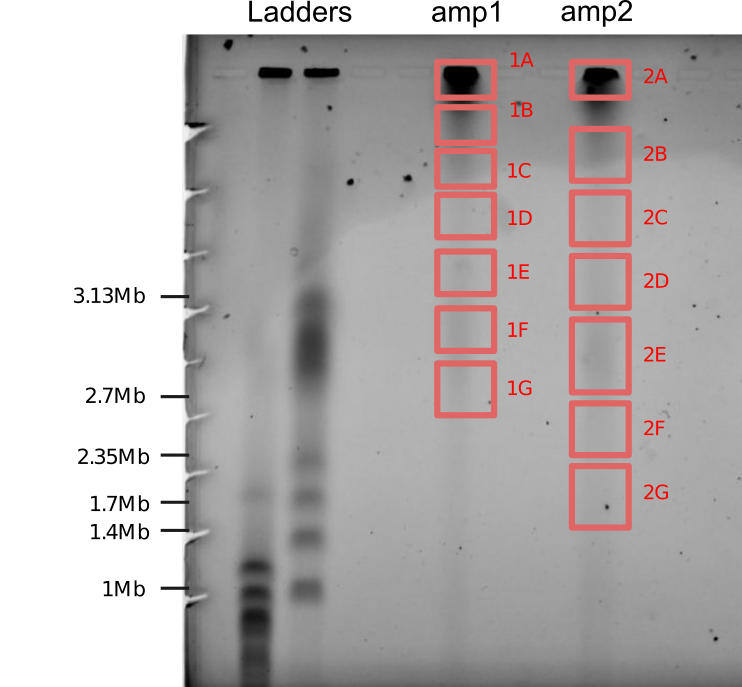
\includegraphics{cc-PFGE-gel}
        \caption{}
        \label{subfig:cc-pfge-gel}
    \end{subfigure}
    \begin{subfigure}{0.49\textwidth}
        \centering
        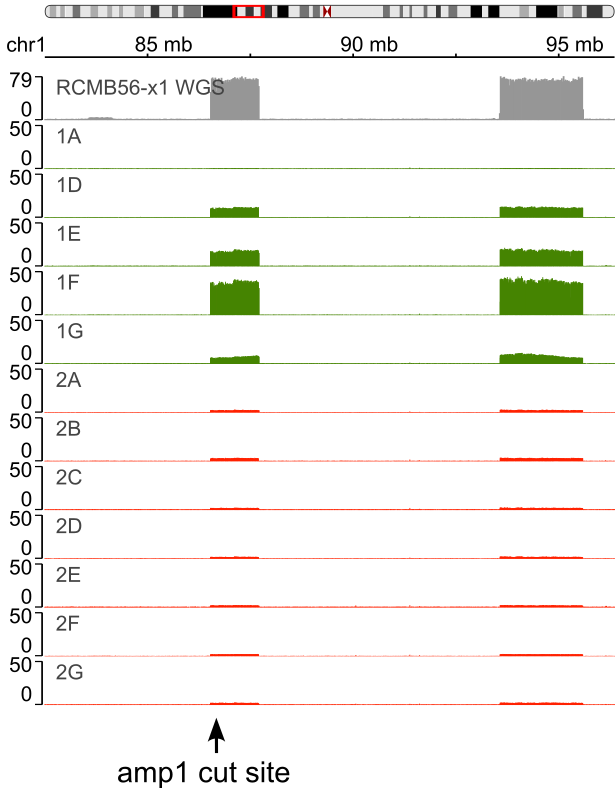
\includegraphics{cc-amp1-igv}
        \caption{}
        \label{subfig:cc-amp1-igv}
    \end{subfigure}
    \begin{subfigure}{0.44\textwidth}
        \centering
        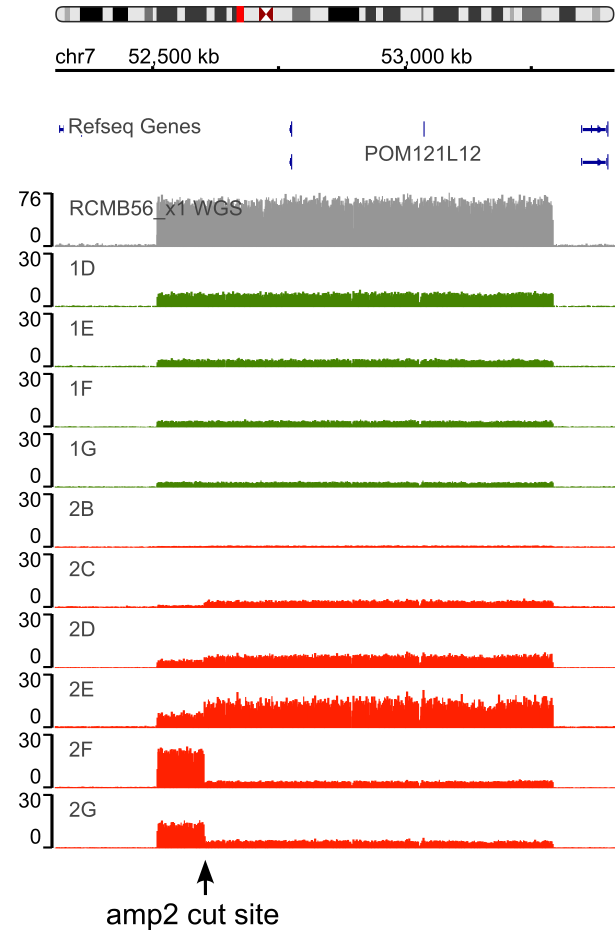
\includegraphics{cc-amp2-igv}
        \caption{}
        \label{subfig:cc-amp2-igv}
    \end{subfigure}
    \begin{subfigure}{0.54\textwidth}
        \centering
        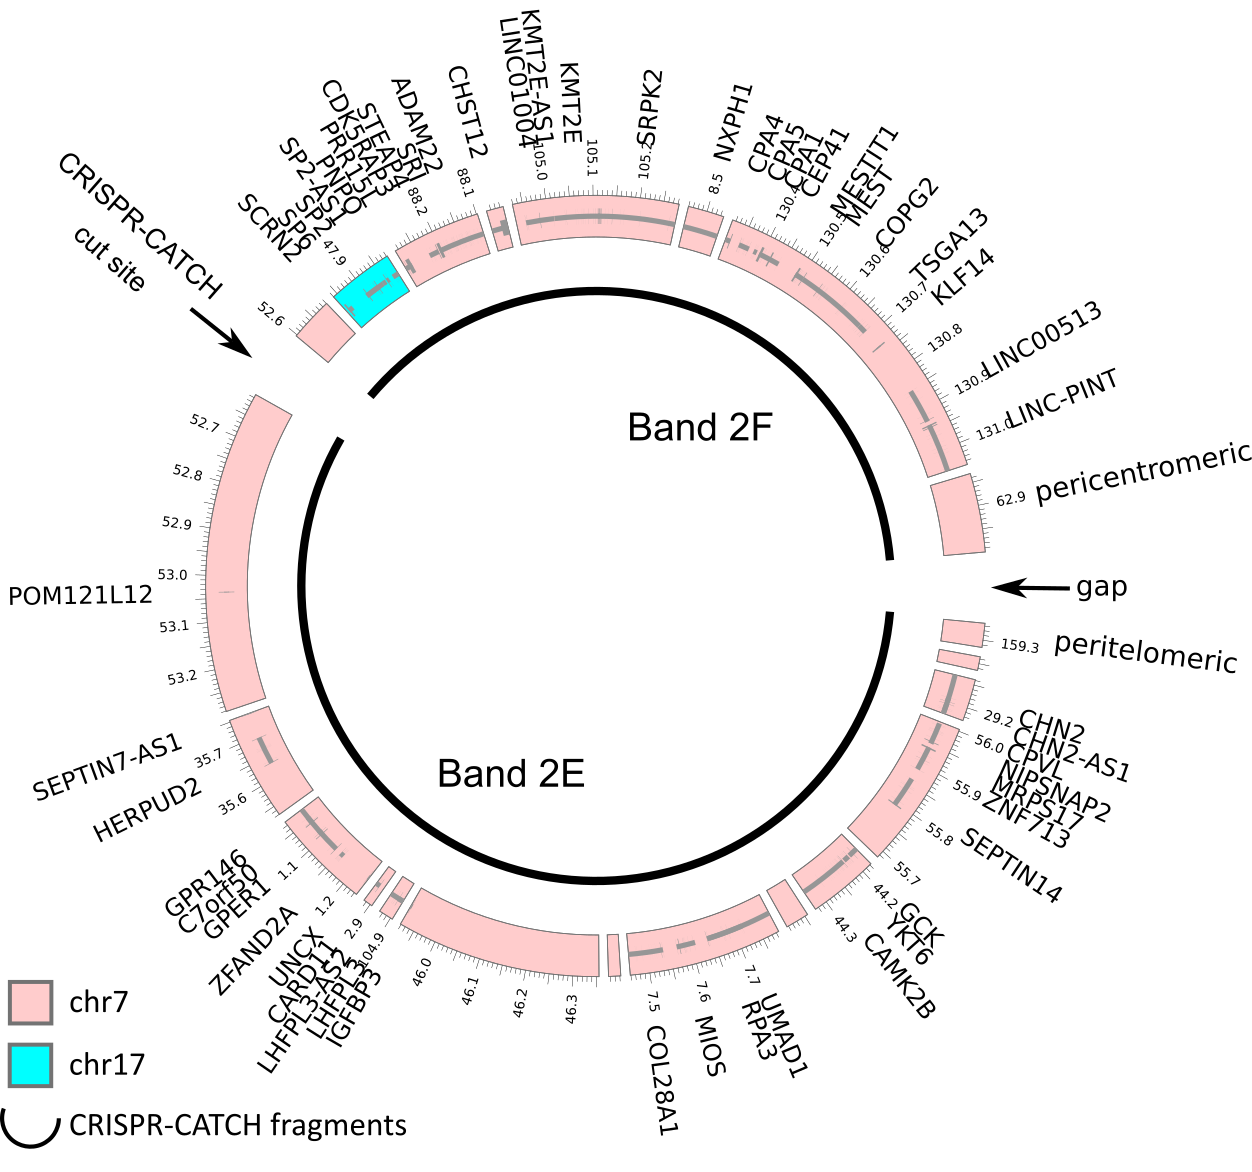
\includegraphics{cc-amp2-circos-map}
        \caption{}
        \label{subfig:cc-amp2-circos-map}
    \end{subfigure}
    \caption[CRISPR-CATCH indicates circular and linear extrachromosomal amplifications in RCMB56 tumors.]{\textbf{CRISPR-CATCH indicates circular and linear extrachromosomal amplifications in RCMB56 tumors.} (\textbf{a}) \gls{uhmw dna} from RCMB56-pdx was cut using CRISPR-Cas9 targeting locations on amp1 or amp2, then sorted by size using \gls{pfge}. Size-sorted bands were then sequenced and aligned to the human reference genome hg38. Circular and chromosomal DNA do not migrate, and are sampled in bands 1A and 1B. (\textbf{b}) \gls{wgs} depth of sequencing coverage of all bands at the amp1 locus. When amp1 is cut (green tracks), \gls{pfge} enriches linear \gls{uhmw dna} mapping to amp1 with a unimodal size distribution centered at $s \approx 3$Mbp (band 1F). When amp1 is not cut (red tracks), no enrichment of amp1 sequences is detected. (\textbf{c}) \gls{wgs} sequencing coverage of all bands at the amp2 locus. When amp2 is not cut (green tracks), \gls{pfge} enriches linear \gls{uhmw dna} mapping to amp2 with size $s \gg 3$Mbp (band 1D). When amp2 is cut (red tracks), \gls{pfge} enriches two distinct fractions of \gls{uhmw dna}, mapping to mutually exclusive fragments of the amp2  assembly and with lengths $s_1 \approx 2.8$Mbp (band 2E) and $s_2 \approx 2.4$Mbp (band 2F). (\textbf{d}) Genomic map of the fragments of amp2 enriched in bands 2E and 2F.}
    \label{fig:cc}
\end{figure}

Visual inspection of the \acrshort{wgs} data also revealed a low-copy gain (gain1) of unknown architecture composed of other segments of chr7 (35Mbp) and chr17 (800kbp). DNA \gls{FISH} imaging of metaphase cells for marker genes \textit{DNTTIP2} (amp1), \textit{KMT2E} (amp2) and \textit{ETV1} (gain1) indicated that amp1 and amp2 are amplified extrachromosomally (Fig. \ref{fig:fish-rcmb56-pdx-metaphase}). To confirm co-occurrence in the same cells, we performed multi-channel FISH imaging for the same markers in interphase cells. We observed distinct fluorescence spots for each gene, indicating that copies of each amplified gene are located on distinct chromatin bodies (Fig. \ref{fig:fish-rcmb56-ht-interphase}). 

\begin{figure}[!h]
    \centering
    \begin{subfigure}{0.32\textwidth}
        \centering
        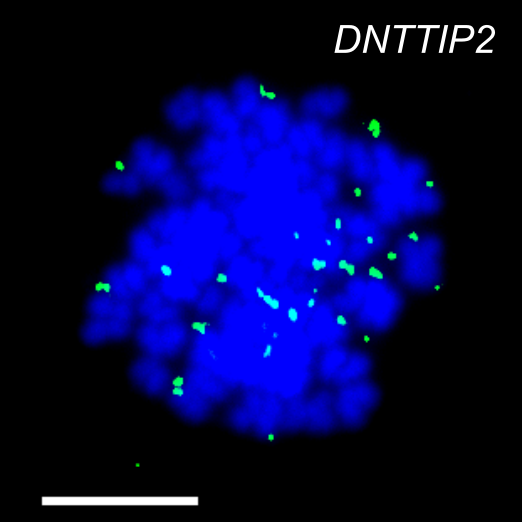
\includegraphics{rcmb56-pdx-dnttip2}
        \caption{}
        \label{subfig:}
    \end{subfigure}
    \begin{subfigure}{0.32\textwidth}
        \centering
        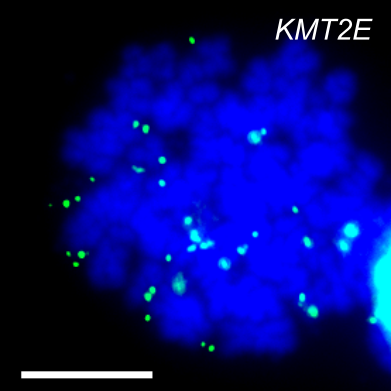
\includegraphics{rcmb56-pdx-kmt2e}
        \caption{}
        \label{subfig:}
    \end{subfigure}
    \begin{subfigure}{0.32\textwidth}
        \centering
        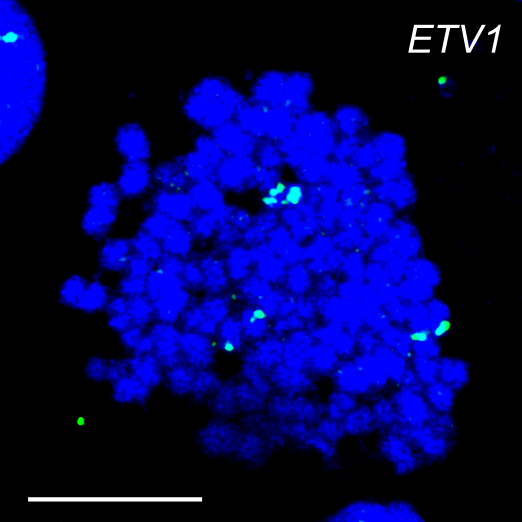
\includegraphics{rcmb56-pdx-etv1}
        \caption{}
        \label{subfig:}
    \end{subfigure}    
    \caption[FISH imaging of amplified marker genes in RCMB56-pdx metaphase cells.]{\textbf{FISH imaging of amplified marker genes in metaphase spreads of RCMB56-pdx nuclei.} (\textbf{a}) Marker gene \textit{DNTTIP2} (amp1). (\textbf{b}) Marker gene \textit{KMT2E} (amp2). (\textbf{c}) Marker gene \textit{ETV1} (gain1). DAPI chromatin stain in blue. Scale bars $10\mu$m.
    }
    \label{fig:fish-rcmb56-pdx-metaphase}
\end{figure}

\begin{figure}
    \centering
    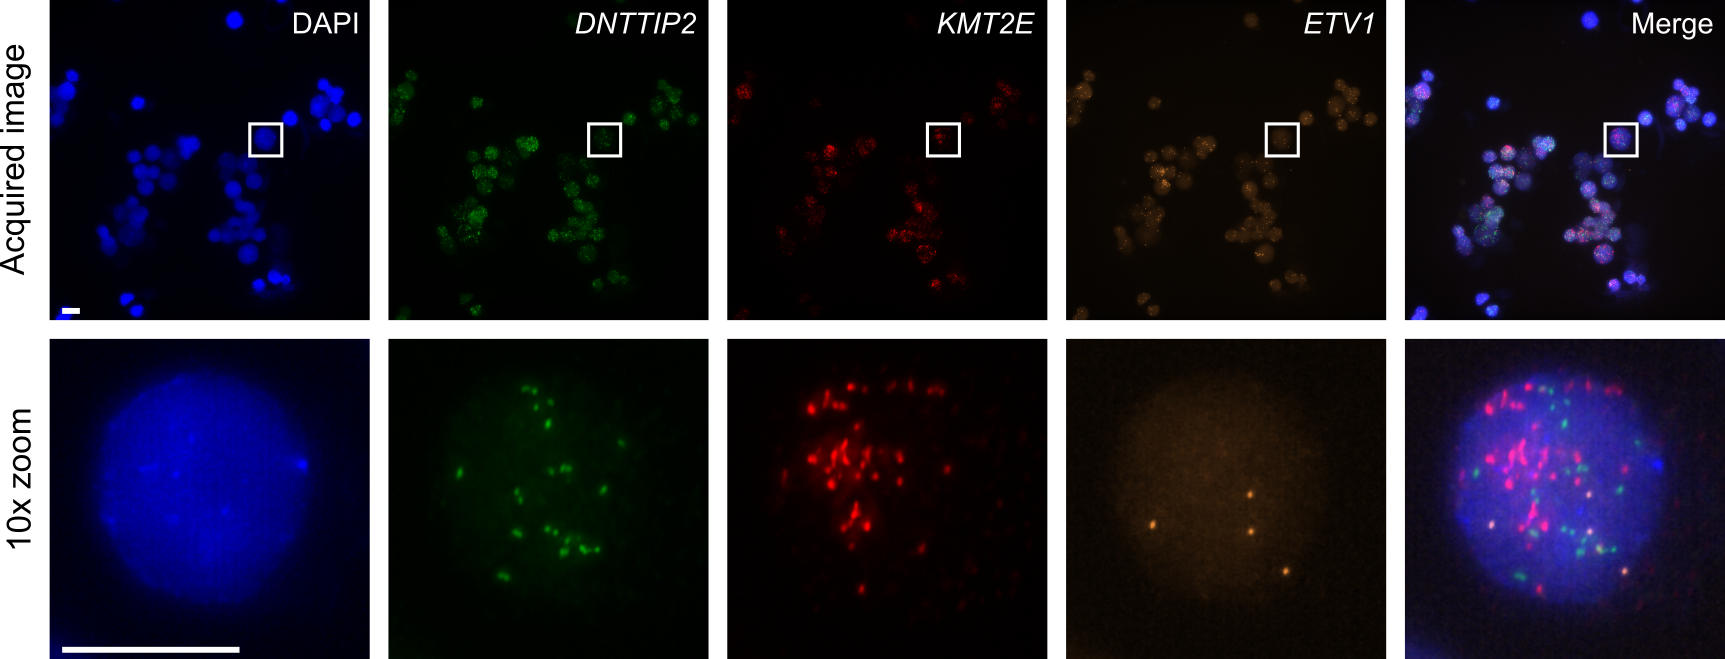
\includegraphics{rcmb56-ht-tricolor}
    \caption[Multi-channel FISH imaging of amplified marker genes in RCMB56-ht interphase cells.]{\textbf{Multi-channel FISH imaging of amplified marker genes in RCMB56-ht interphase cells.} Example image shown on top row, 10x zoom of an example single cell on bottom row. Columns from left to right: DAPI channel (chromatin), \textit{DNTTIP2} (amp1), \textit{KMT2E} (amp2), \textit{ETV1} (gain1), merge of all channels. Marker gene copies are spatially independent, indicating distinct amplifications of all 3 markers in the same cells. 
    }
    \label{fig:fish-rcmb56-ht-interphase}
\end{figure}

\subsection{MB patient tumors with ecDNA exhibit high intratumoral copy number heterogeneity.}
Substantial intratumoral copy number heterogeneity is expected in an ecDNA+ tumor due to random segregation of ecDNA during mitosis, driving tumor evolution and treatment resistance \cite{Lange_2021}.  To determine the extent of ecDNA copy number heterogeneity in patient MB tumors, we established an automated image analysis pipeline to estimate the distributions of copy number per cell in interphase FISH microscopy imaging (see Methods \ref{methods:fish}) and applied it to four primary MB tumors harboring ecDNA: MB036 (\textit{MYCN}), MB177 (\textit{MYCN}), MB268 (\textit{MDM4}), and RCMB56 (\textit{DNTTIP2}, \textit{KMT2E}, \textit{ETV1}). The estimated copy number per cell of all ecDNA-amplified marker genes had significantly greater mean (Wilcoxon test) and variance (Levene's test) than the ecDNA- cell line COLO320-HSR (Fig. \ref{fig:fish-heterogeneity}) which includes \textit{MYC} on a chromosomal amplification \cite{hung_2021}. These results from human MB tumors are consistent with high copy number heterogeneity observed in human cancer cell lines with ecDNA \cite{Lange_2021}. In each primary tumor analyzed, ecDNA was amplified (copy number greater than 5) in only a subset of cells (22-41\%, Supplementary Table 5 of \cite{Chapman}). 

\begin{figure}[!h]
    \centering
    \centerline{%
    \begin{subfigure}{1.1\textwidth}
        \centering
        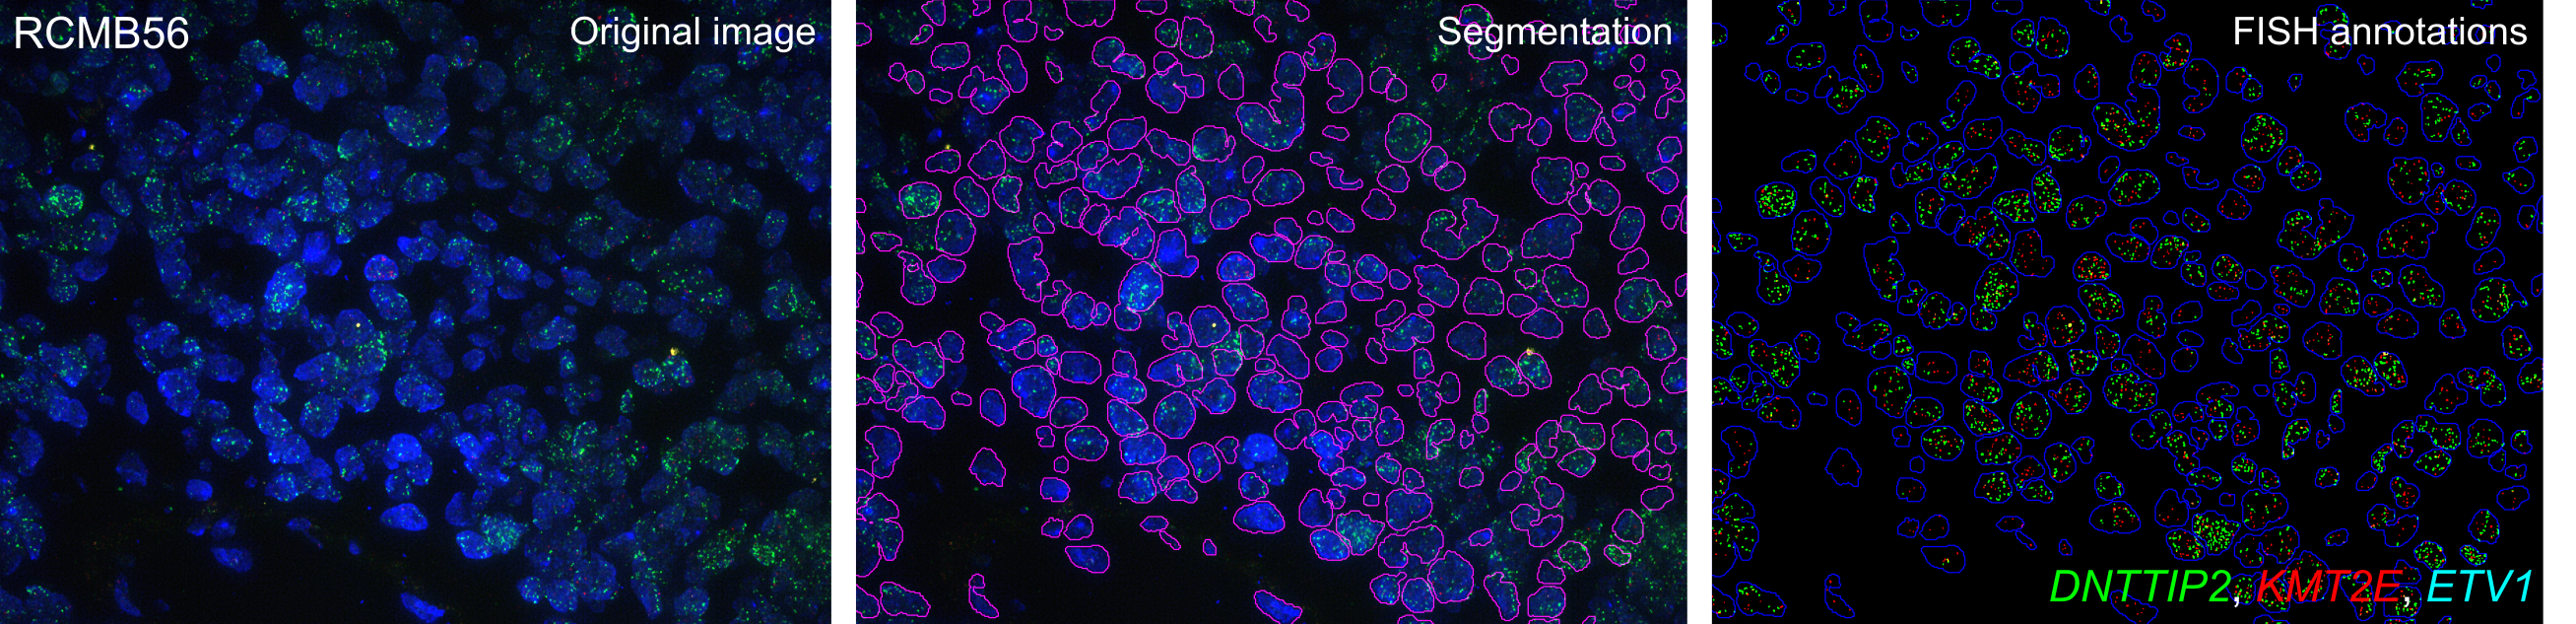
\includegraphics{rcmb56-ht-segmentation}
        \caption{}
        \label{subfig:fish-segmentation}
    \end{subfigure}%
    }
    \centerline{%
    \begin{subfigure}{1.1\textwidth}
        \centering
        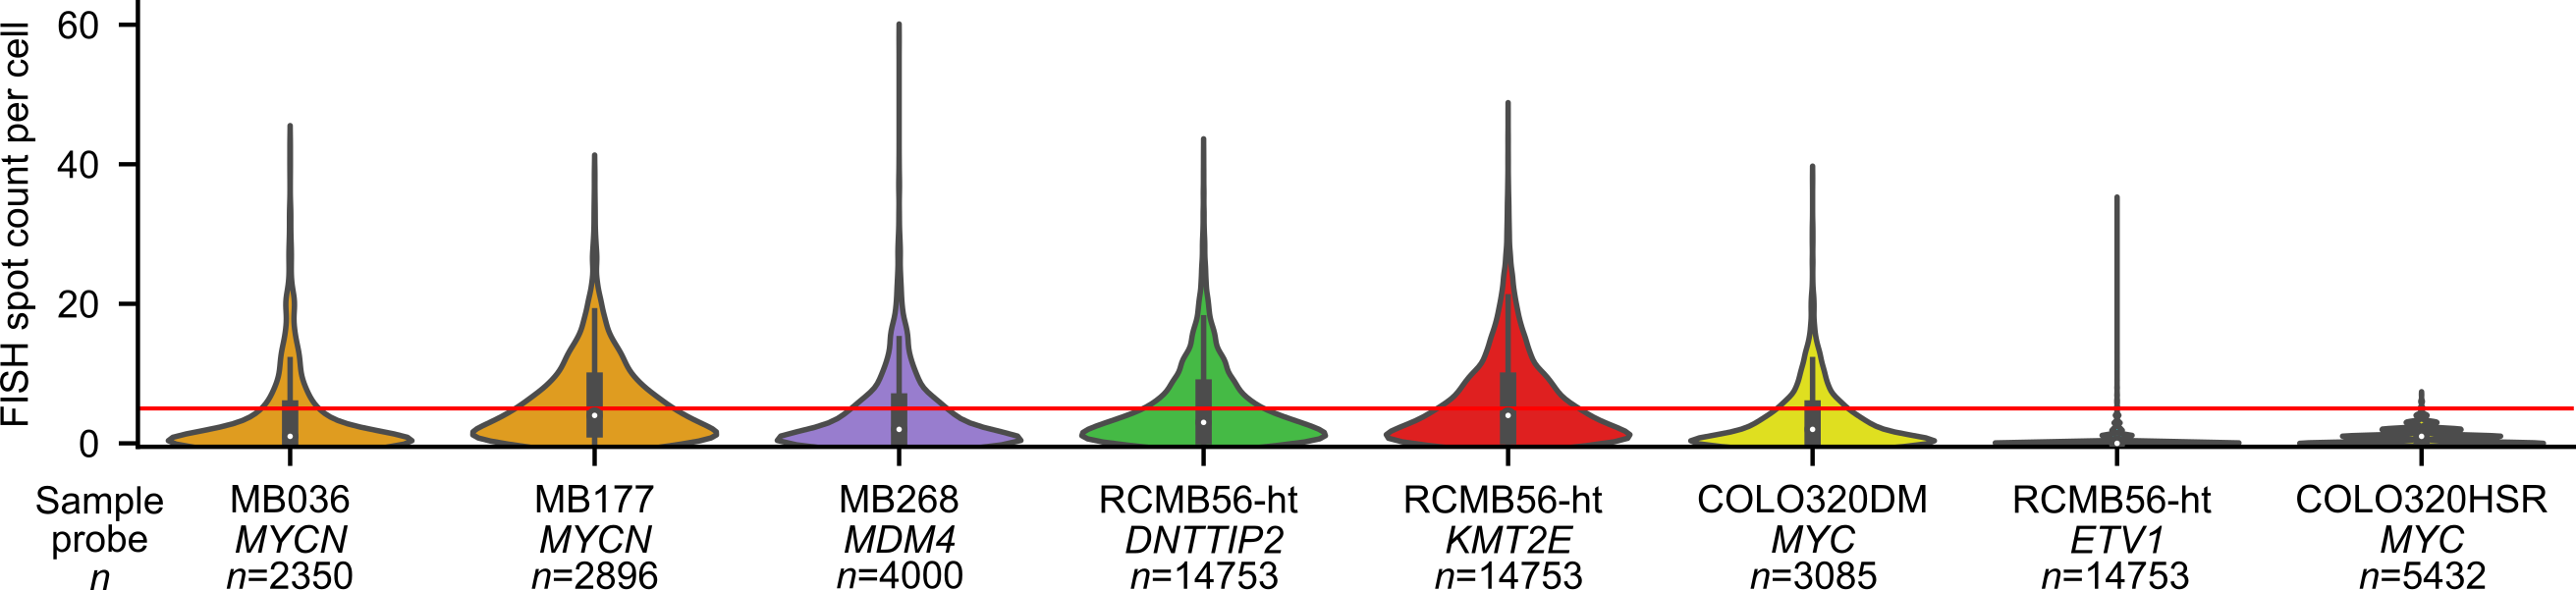
\includegraphics{violin-fish-counts}
        \caption{}
        \label{subfig:violin-fish-counts}
    \end{subfigure}%
    }
    \caption[Copy number estimation of ecDNA in single cells from FISH microscopy]{\textbf{Copy number estimation of ecDNA in single cells from FISH microscopy.} (\textbf{a}) Example output of automated image analysis pipeline. Segmentation: nuclear boundaries were detected from the DAPI channel image using NuSeT \cite{nuset}. FISH annotations: The number of FISH foci was inferred using ecSeg-i \cite{ecseg}. (\textbf{b}) Estimated copy counts for amplified foci on ecDNA and other copy gains. Red line indicates $n\geq5$, the threshold whereupon a cell was classified as amplified.
    }
    \label{fig:fish-heterogeneity}
\end{figure}

\par To determine whether copy number heterogeneity of an ecDNA+ tumor is accompanied by transcriptional heterogeneity, we analyzed 2,762 single nuclei from frozen tissue of RCMB56-ht using a multiome snRNA+ATAC-seq assay (10X Genomics) to profile transcriptomes and accessible chromatin of the same individual cells. Consistent with previous findings in bulk samples \cite{Turner_2017,Wu_2019} RCMB56-ht single nucleus ATAC-seq (snATAC-seq) sequencing coverage was enriched at the amp1 and amp2 loci at the aggregate level, and also in individual cells (Fig. \ref{subfig:scATAC-coverage}). To detect focal amplifications in single nuclei, we performed Monte Carlo permutation tests comparing snATAC-seq read density at the amplicon locus to that at random locations elsewhere in the genome (excluding blacklisted regions, see Methods \ref{methods:ssgsea}). Z-score normalized read density at the amp1 and amp2 loci had greater mean and variance than at gain1 (Fig. \ref{subfig:violin-scatac-coverage}), consistent with the copy number heterogeneity we observed in the interphase FISH data. We conservatively estimate that at least 224 out of 2762 (8\%, FDR $q < 0.10$) cells contained amp1 or amp2 (ecDNA+ cells). Of these, both amp1 and amp2 were detected together in only a minority of cells (72 out of 224, 32\%) (Fig. \ref{subfig:venn-ecDNA+cells}). Thus, evidence from quantitative FISH microscopy and multiome single-cell sequencing show that only a fraction of tumor cells in ecDNA+ MB tumors harbor high-copy ecDNA, and that these have highly variable copy numbers of extrachromosomal amplifications. 

\begin{figure}[!h]
    \centering
    \centerline{%
    \begin{subfigure}{1.2\textwidth}
        \centering
        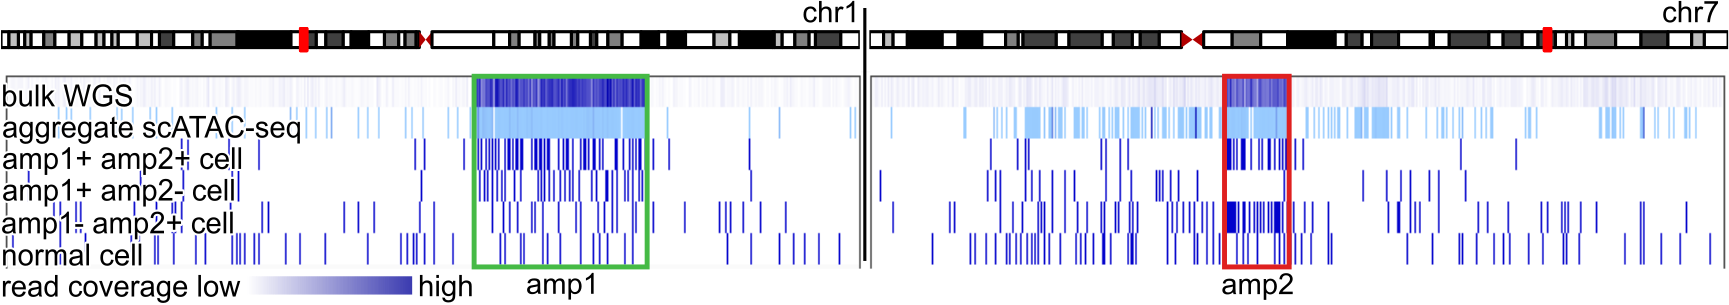
\includegraphics{scATAC-coverage}
        \caption{}
        \label{subfig:scATAC-coverage}
    \end{subfigure}%
    }
    \begin{subfigure}{.49\textwidth}
        \centering
        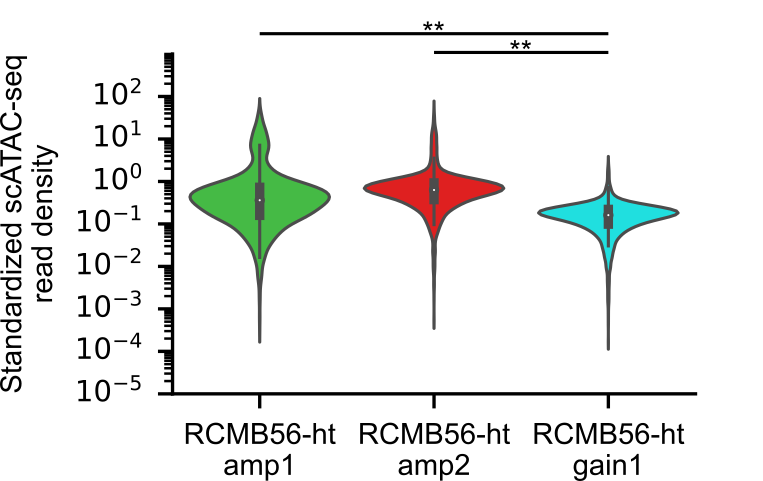
\includegraphics{scATAC-coverage-violin}
        \caption{}
        \label{subfig:violin-scatac-coverage}
    \end{subfigure}
    \begin{subfigure}{.49\textwidth}
        \centering
        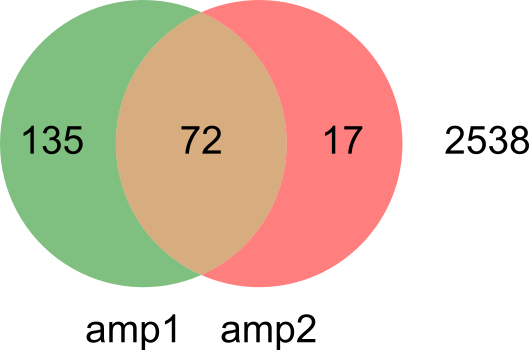
\includegraphics{rcmb56-ht-ecDNA+classifications}
        \caption{}
        \label{subfig:venn-ecDNA+cells}
    \end{subfigure}
    \caption[Detection of ecDNA in in single cells from single-cell ATAC-seq of RCMB56-ht.]{\textbf{Detection of ecDNA in in single cells from single-cell ATAC-seq of RCMB56-ht.} (\textbf{a}) Mapped read density of sequencing modalities at RCMB56 amp1 and amp2 loci. Tracks from top to bottom: bulk \gls{wgs}, aggregate scATAC-seq across all cells, and scATAC-seq of individual cells. (\textbf{b}) Distribution of Z-score normalized read coverage at the amp1, amp2, and gain1 loci. ** $p < 0.005$, Mann-Whitney test. (\textbf{c}) Sets of RCMB56 cells identified as harboring high-copy amplification of amp1 and amp2. Monte Carlo permutation test, $q < 0.05$.
    }
    \label{fig:scatac-heterogeneity}
\end{figure}

\subsection{ecDNA+ and ecDNA- tumor cell populations in the same tumor have distinct transcriptional profiles.}
Clustering single cells using the Weighted Nearest Neighbors algorithm (WNN, \cite{seurat_4}) placed the majority of ecDNA+ cells in a single cluster with distinct transcriptional and epigenetic features (Fig. \ref{fig:rcmb56-ht-clustering}). As expected, cells in the ecDNA+ cluster overexpressed \textit{DNTTIP2} ($q < 0.001$, Wilcoxon Rank Sum test) and \textit{KMT2E} ($q < 0.001$), the marker genes amplified on amp1 and amp2. Compared with other tumor and normal cells, ecDNA+ tumor cells also overexpressed \textit{GLI2} ($q < 0.001$), a known mediator of SHH-mediated transcription and a marker for SHH \gls{MB}, despite \textit{GLI2} not being affected by copy number alteration in this tumor. (Fig. \ref{subfig:clustering-exp-dotplot}, Supplementary Table 6 of \cite{Chapman}). To further investigate the relationship between ecDNA copy number and transcription, we estimated first, ecDNA copy number in single cells (z-scores), and second, the transcriptional activity of genes amplified on ecDNA in each cell (ssGSEA \cite{ssGSEA_2009} scores, see Methods \ref{methods:ssgsea}). As expected, ssGSEA scores were positively correlated with z-scores, indicating increased transcription of ecDNA-amplified genes with increasing ecDNA copy number (Fig. \ref{fig:ssgsea-x-zscores}). 

\begin{figure}[!h]
    \centering
    \begin{subfigure}{.49\textwidth}
        \centering
        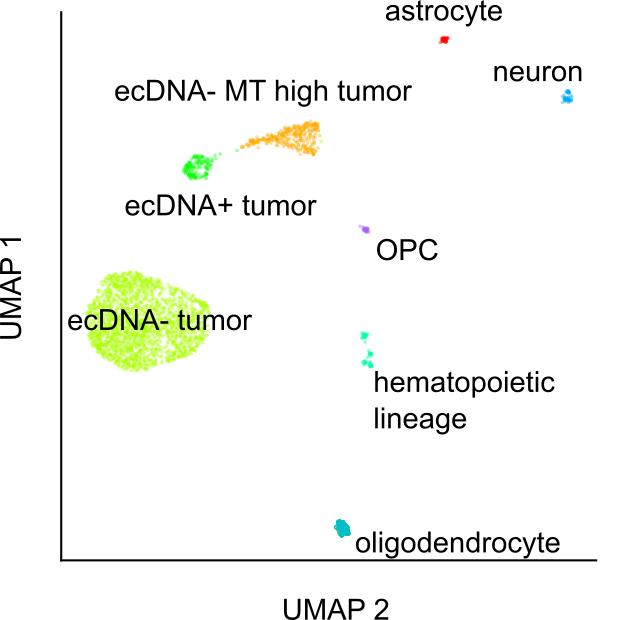
\includegraphics{rcmb56-ht-celltype-umap-v2}
        \caption{}
        \label{subfig:clustering-celltypes}
    \end{subfigure}
    \begin{subfigure}{.49\textwidth}
        \centering
        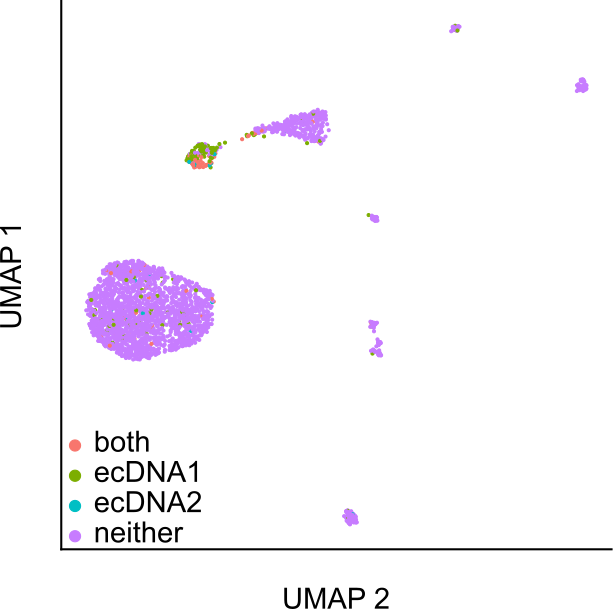
\includegraphics{rcmb56-ht-ecDNA-status-umap}
        \caption{}
        \label{subfig:clustering-ecDNA-status}
    \end{subfigure}
    \begin{subfigure}{.49\textwidth}
        \centering
        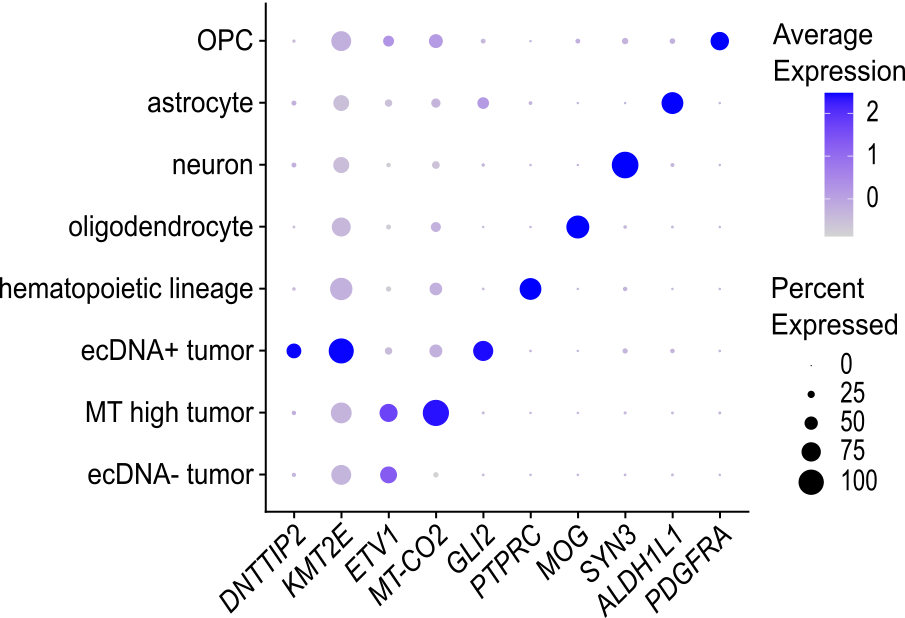
\includegraphics{rcmb56-ht-dotplot}
        \caption{}
        \label{subfig:clustering-exp-dotplot}
    \end{subfigure}
    \caption[RCMB56 ecDNA+ cells express a distinct transcriptional and epigenetic profile.]{\textbf{RCMB56 ecDNA+ cells express a distinct transcriptional and epigenetic profile.} (\textbf{a}) UMAP projection of 2,762 RCMB56-ht cells were clustered by joint transcriptional and epigenetic profiles using the WNN algorithm \cite{seurat_4}. ecDNA- tumor: cells harboring other structural variants but not enriched for ecDNA (see also Fig. \ref{fig:rcmb56-ht-infercnv}). ecDNA- MT high: ecDNA- tumor cells with high expression of mitochondiral genes. Normal cells were identified by expression of marker genes. (\textbf{b}) UMAP projection of RCMB56-ht cells labelled by high-copy focal amplification of ecDNA, identifed by depth of scATAC-seq coverage at ecDNA loci. (\textbf{c}) Transcription of marker genes in single cells of RCMB56-ht.  
    }
    \label{fig:rcmb56-ht-clustering}
\end{figure}

\begin{figure}[!h]
    \centering
    \begin{subfigure}{.49\textwidth}
        \centering
        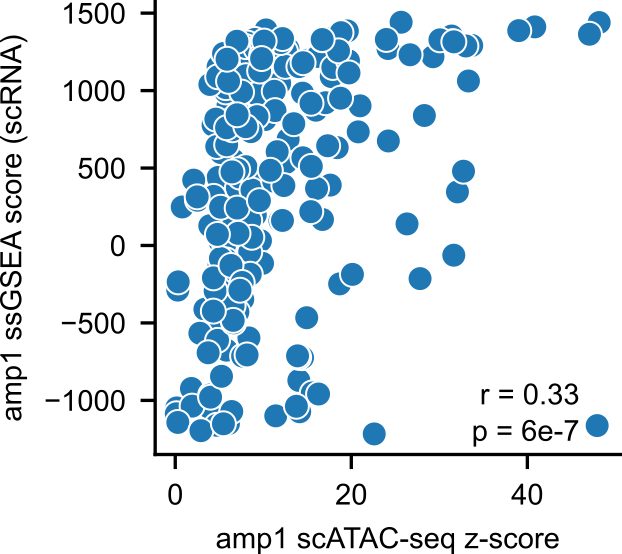
\includegraphics{ssgsea1-x-zscore1}
        \caption{}
    \end{subfigure}
    \begin{subfigure}{.49\textwidth}
        \centering
        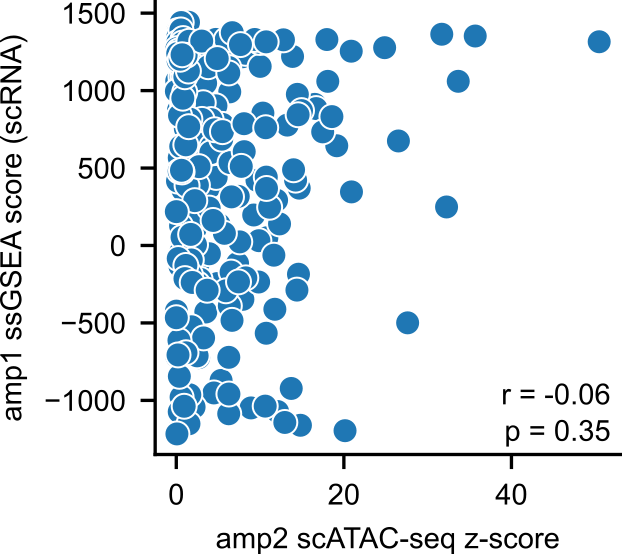
\includegraphics{ssgsea1-x-zscore2}
        \caption{}
    \end{subfigure}
    \begin{subfigure}{.49\textwidth}
        \centering
        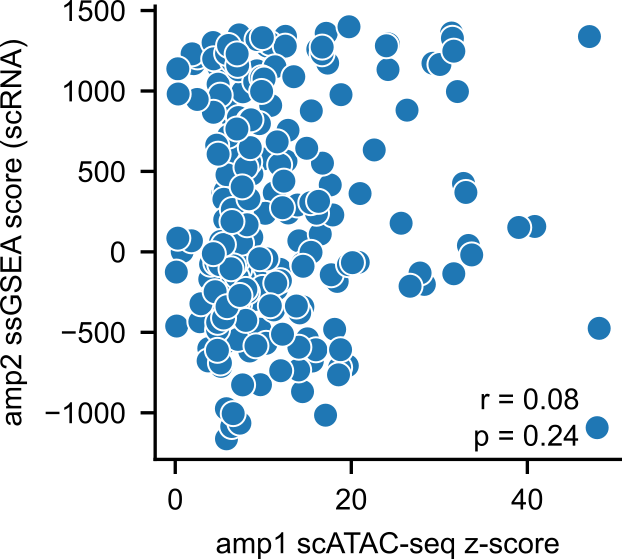
\includegraphics{ssgsea2-x-zscore1}
        \caption{}
    \end{subfigure}
    \begin{subfigure}{.49\textwidth}
        \centering
        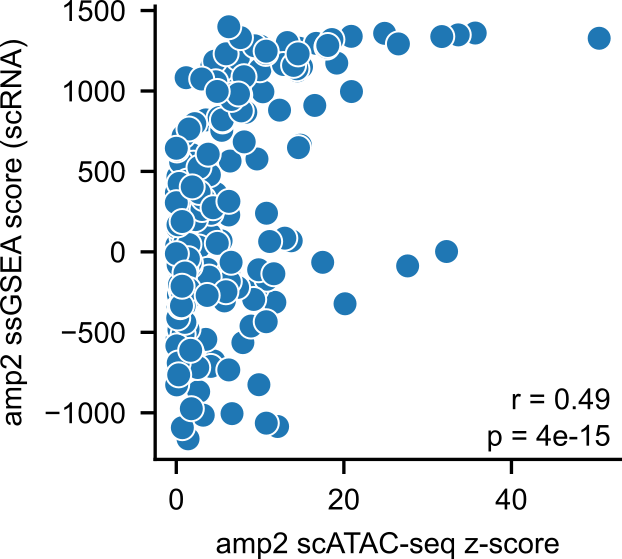
\includegraphics{ssgsea2-x-zscore2}
        \caption{}
    \end{subfigure}
    \caption[ecDNA copy number is associated with gene expression of ecDNA-amplified genes.]{\textbf{ecDNA copy number is associated with gene expression of ecDNA-amplified genes.} Pearson correlations between copy number at the amplified locus (z-scores) and transcriptional activity of amplified genes (ssGSEA scores). Copy number of amp1 is associated with transcription of amp1-amplified genes, but not with transcription for amp2-amplified genes. Conversely, copy number of amp2 is associated with amp2-amplified, but not amp1-amplified, gene expression. 
    }
    \label{fig:ssgsea-x-zscores}
\end{figure}

In addition to the ecDNA+ tumor cells, we identified two other clusters of tumor cells not enriched for ecDNA and with low expression of the amp1 and amp2 marker genes, one of which strongly expressed mitochondrial genes (`ecDNA-' and `ecDNA- MT high'), as well as normal cells such as astrocytes, oligodendrocytes and cells from the hematopoietic lineage (Fig. \ref{subfig:clustering-exp-dotplot}). Normal cell types were annotated by cell cluster-specific expression of known marker genes. Genomic copy number estimation from snRNA-seq confirms that normal cells had stable genomes whereas the tumor cells were characterized by copy-number alterations (Fig. \ref{fig:rcmb56-ht-infercnv}). 

\begin{figure}[!h]
    \centering
    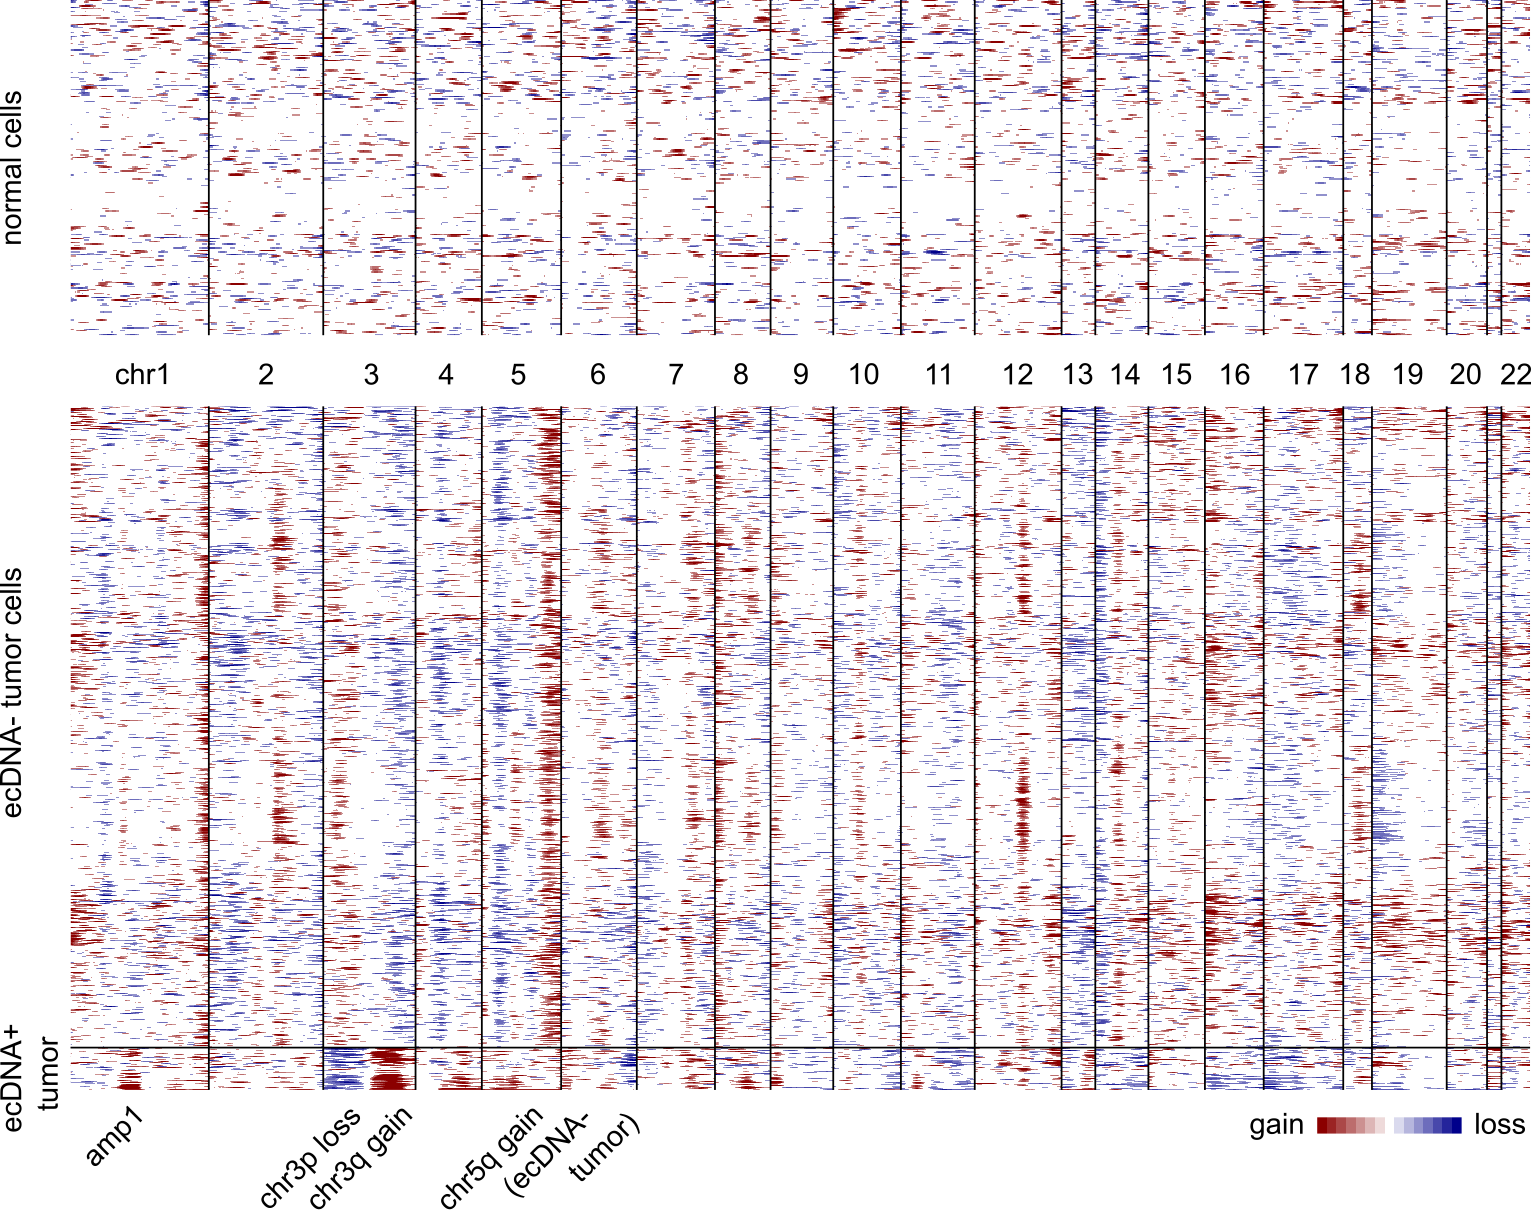
\includegraphics{rcmb56-ht-infercnv}
    \caption[Aneuploidy estimated from single-cell transcriptomes of 2,762 cells from RCMB56-ht]{\textbf{Aneuploidy estimated from single-cell transcriptomes of 2,762 cells from RCMB56-ht} using inferCNV \cite{inferCNV_2019}. Diploid cells comprising the astrocyte, neuron, OPC, hematopoietic and oligodendrocyte cell clusters comprised the reference set of normal cells. The cluster enriched for high-copy ecDNA is annotated. This cluster also uniquely harbors chr3p deletion and chr3q gain.}
    \label{fig:rcmb56-ht-infercnv}
\end{figure}

\subsection{A PDX model resembles ecDNA+ cells of its origin human tumor.}

Patient-derived xenografts (PDX) and cell lines have been used as preclinical models for identification and testing of compounds for new targeted therapies for MB \cite{rusert_2020}. To test whether cells in a PDX faithfully model ecDNA in the corresponding human tumor, we applied multiome scRNA+ATAC-seq to fresh tissue from passage 1 of the RCMB56-pdx model. In contrast to RCMB56-ht, nearly every human cell in the RCMB56-pdx sample contained ecDNA (9608 out of 9,620, 99.96\%, $q < 0.10$) (Fig. 4f, Supplementary Fig. 7b). The majority of these contained both amp1 and amp2 (8554 out of 9608, 89\%). Batch-correction and dimensionality reduction on the unified set of transcriptomes from both samples, using the Conos package \cite{conos_2019}, indicates that the cells of the PDX are transcriptionally similar to ecDNA+ cells in RCMB56-ht, and distinct from all other RCMB56-ht cells (Fig. \ref{fig:rcmb56-pdx-clustering}). We then asked whether the human tumor ecDNA+ cell subpopulation harbored additional identifying genomic alterations which could be confirmed in the PDX. Genomic copy number estimation from the scRNA-seq data indicated that tumor cells of the RCMB56-ht ecDNA+ cluster uniquely harbored chr3p deletion and chr3q duplication but not chr5q duplication (Fig. \ref{fig:rcmb56-ht-infercnv}). Cells from RCMB56-pdx universally harbored the same alterations (Fig. \ref{fig:rcmb56-pdx-infercnv}). These results indicate that the PDX tumor RCMB56-pdx is a clonal expansion of the ecDNA+ cells of the human tumor RCMB56-ht. 

\begin{figure}[!h]
    \centering
    \begin{subfigure}{.49\textwidth}
        \centering
        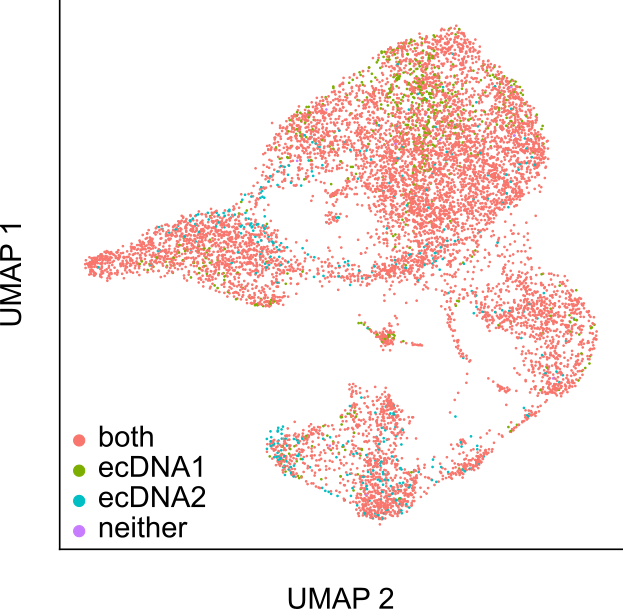
\includegraphics{rcmb56-pdx-ecDNA-status-umap}
        \caption{}
    \end{subfigure}
    \begin{subfigure}{.49\textwidth}
        \centering
        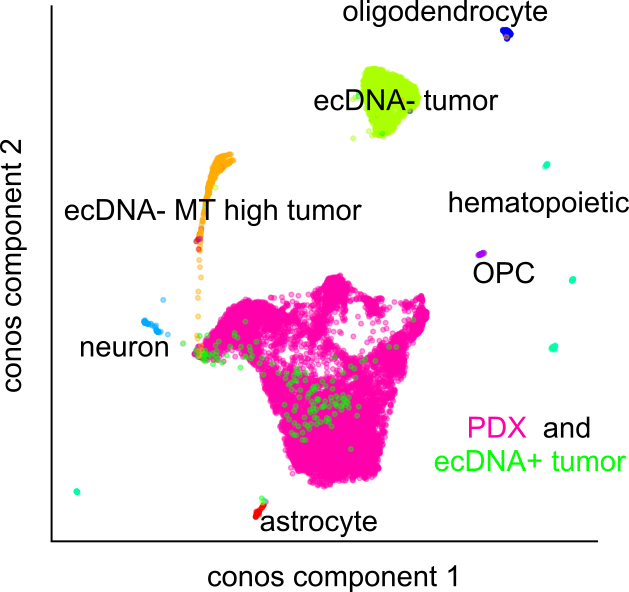
\includegraphics{rcmb56-pdx-conos}
        \caption{}
        \label{subfig:conos}
    \end{subfigure}
    \caption[High-copy ecDNA is universally present in 9,620 RCMB56-pdx cells.]{\textbf{High-copy ecDNA is universally present in 9,620 RCMB56-pdx cells.} (\textbf{a}) Low-dimensional UMAP embedding of 9,620 RCMB56-pdx accessible chromatin and transcriptomes, annotated by ecDNA detected by scATAC-seq. (\textbf{b}) Low-dimensional embedding of 9,620 RCMB56-pdx and 2,762 RCMB56-ht transcriptomes, integrated and batch-corrected using Conos \cite{conos_2019}. PDX cells (pink) overlap ecDNA+ cells from the patient tumor, but are distinct from other RCMB56-ht cell clusters.}
    \label{fig:rcmb56-pdx-clustering}
\end{figure}

\begin{figure}[!h]
    \centering
    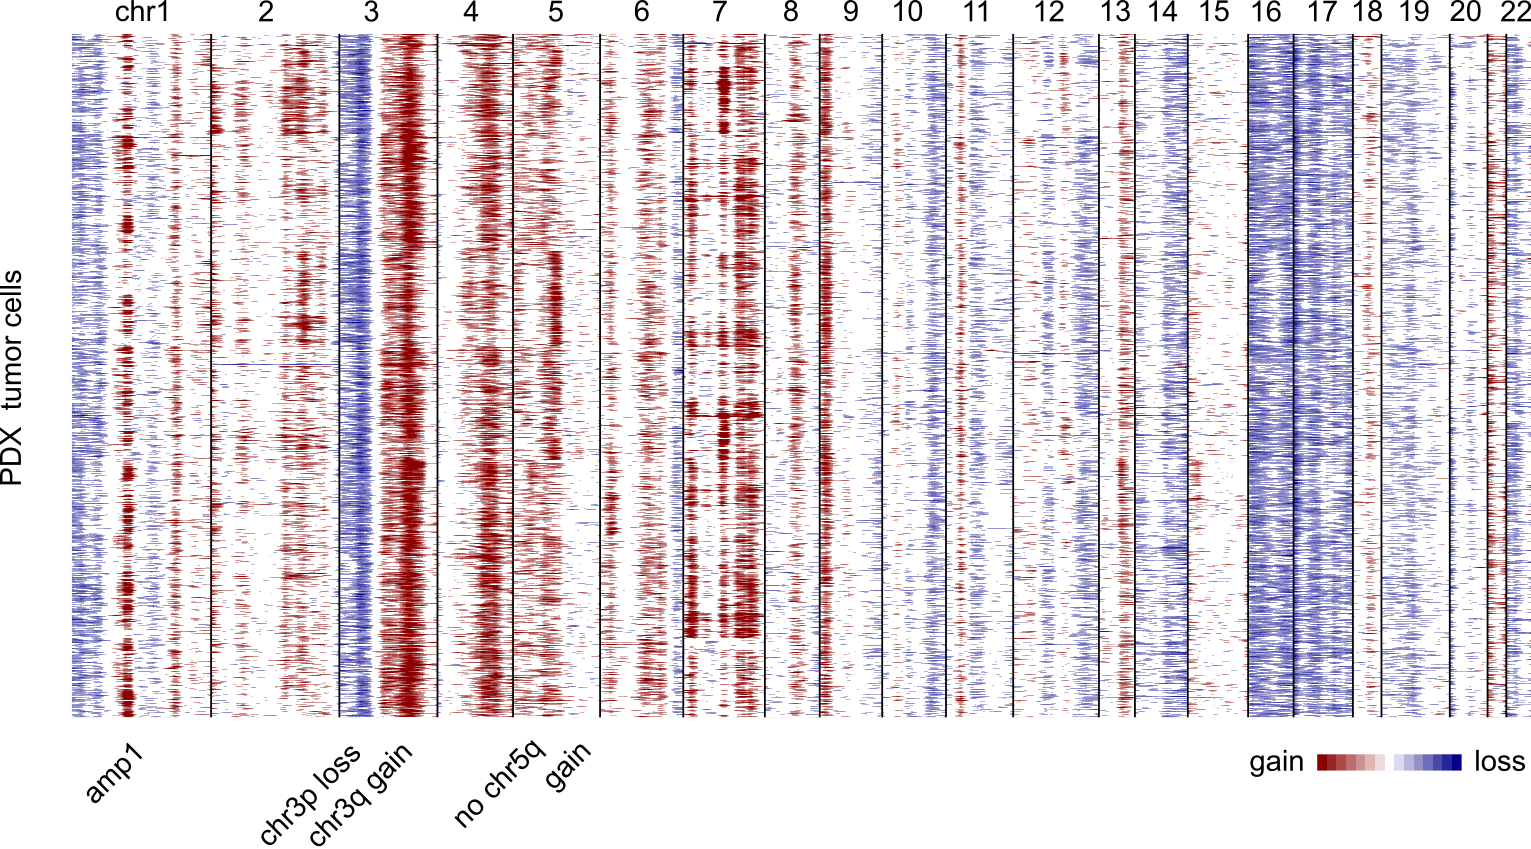
\includegraphics{rcmb56-pdx-infercnv}
    \caption[Aneuploidy estimated from single-cell transcriptomes of 9,620 cells from RCMB56-pdx]{\textbf{Aneuploidy estimated from single-cell transcriptomes of 9,620 cells from RCMB56-pdx} using inferCNV \cite{inferCNV_2019}. PDX cells univerally harbor the chromosomal copy gain (chr3q) and loss (chr3p) which uniquely identify ecDNA+ cells in the RCMB56-ht human tumor (Fig. \ref{fig:rcmb56-ht-infercnv}).
    }
    \label{fig:rcmb56-pdx-infercnv}
\end{figure}

\subsection{The relapsed RCMB56 patient tumor karyotype was present in a subpopulation of ecDNA+ cells in the primary.}
Following maximal resection, the RCMB56 primary tumor had been treated according to the standard of care with high-dose craniospinal proton therapy and chemotherapy including cisplatin, cyclophosphamide, and vincristine \cite{rusert_2020}. Two years after initial diagnosis, however, the RCMB56 tumor recurred and a second surgical resection was performed. WGS data from \gls{FFPE} tissue of the relapsed tumor (RCMB56-r1) indicated copy-number amplification at the amp1 locus but not the amp2 locus (data not shown). Computational reconstruction using \gls{AA} confirmed that the amp1 sequence remained largely unchanged. Following WGS, no tissue remained of the relapsed tumor for further analysis. Thus, although we cannot rule out that amp2 was present in an area of the relapsed tumor which was not sampled, we observe amp1 but no evidence of amp2 in the RCMB56 relapsed patient tumor.

\section{Discussion}
Analyses of the p53-mutant SHH tumor RCMB56-ht reveal intratumoral heterogeneity not present in subsequent longitudinal biopsies of the same tumor. Sequence assembly, from whole genome short-read sequencing, optical genome mapping on long reads, and CRISPR-CATCH, reconstructs two distinct high-copy extrachromosomal focal amplifications, one from 3 segments of chr1 and the other from 20 segments of chr7 and chr17. Analyses of FISH microscopy and single-cell sequencing of RCBM56-ht tissue concur that both amplicons may be found in the same tumor cells, and that amplicon copy number is highly variable between cells. Further analysis of multi-omic single-cell sequencing data reveals that tumor cells with high-copy ecDNA expressed a distinct transcriptional and epigenetic program, including \textit{GLI2}, a marker of malignant SHH subgroup MB. Thus, the RCMB56 patient tumor comprised a population of cells with heterogeneous ecDNA sequences, ecDNA copy number, and cell states. 

\par Although ecDNA+ and ecDNA- tumor cells coexisted in RCMB56-ht, the presence or absence of ecDNA became fixed in subsequent tumors descended from the primary tumor. In the relapsed tumor RCMB56-r1, resected 2 years after original diagnosis, we find amp1 but no evidence of amp2. In RCMB56-pdx, amp1 and amp2 are near-univerally present, indicating loss of the ecDNA- tumor cell subpopulation during engraftment. Thus, in either RCMB56 tumor, we observe substantial changes of intratumoral heterogeneity of ecDNA following a strong selective pressure. It remains to be seen whether similar changes in ecDNA+ cell populations occur in other patient tumors during tumor progression, or in other PDX models under selective pressure.

\par Data from multiple modalities confirm the circular extrachromosomal sequence of amp1, but not amp2. Whereas sequence assembly from \gls{wgs} and \gls{ogm} data fully reconstruct the circular amp1 sequence, the same data map a linear amp2 sequence assembly, with ends mapping to pericentromeric and peritelomeric regions of chr7. Cutting circular amp1 by CRISPR-CATCH yields linear DNA of the approximate length of the amp1 assembly, but cutting amp2 results in 2 fractions of linear DNA, whose lengths and sequences sum to the length and sequence of the amp2 assembly. In chapter 3, we will observe in Hi-C data that the ends of the amp2 assembly do not co-localize spatially. Nevertheless, amp2 appears a high-copy extrachromosomal amplification in FISH imaging, and the copy number distribution per cell resembles that of circular amp1. The base-resolution sequences of the amp2 assembly ends remain an intriguing unresolved question, and may shed light on whether stable linear extrachromosomal amplification can arise in human tumors.

% \par Short concluding comments. What is the one-sentence takeaway?

\section{Methods}
\subsubsection{Animals}
NOD-SCID IL2R$\gamma$ null (NSG) mice used for intracranial human tumor transplantation were purchased from The Jackson Laboratory (\#005557). Mice were bred and maintained in the animal facilities at the Sanford Consortium for Regenerative Medicine. All experiments were performed in accordance with national guidelines and regulations, and with the approval of the animal care and use committees at the Sanford Burnham Prebys Medical Discovery Institute and University of California San Diego (San Diego, CA, USA).

\subsubsection{Establishment and maintenance of \acrshort{rcmb56-pdx}}
The \acrlong{rcmb56-pdx} model was established by implanting 0.5-1x106 dissociated patient tumor cells directly into the cerebellum of NSG mice. Subsequent tumors were harvested from mice, dissociated and reimplanted into new NSG mice without \textit{in vitro} passaging. \textit{Ex vivo} experiments were performed with PDX RCMB56 cells of \textit{in vivo} passage 1 (x1).

\subsection{Optical genome mapping data collection and processing}
Ultra-high molecular weight (UHMW) DNA was extracted from frozen cells preserved in DMSO following the manufacturer's protocols (Bionano Genomics, USA). Cells were digested with Proteinase K and RNAse A. DNA was precipitated with isopropanol and bound with nanobind magnetic disks. Bound UHMW DNA was resuspended in the elution buffer and quantified with Qubit dsDNA assay kits (ThermoFisher Scientific).
\par DNA labeling was performed following manufacturer's protocols (Bionano Genomics, USA). Standard Direct Labeling Enzyme 1 (DLE-1) reactions were carried out using 750 ng of purified UHMW DNA. The fluorescently labeled DNA molecules were imaged sequentially across nanochannels on a Saphyr instrument. A genome coverage of at least 400x was achieved for all samples. 
\par \textit{De novo} assemblies of the samples were performed with Bionano's \textit{De Novo} assembly Pipeline (DNP) using standard haplotype aware arguments (Bionano Solve v3.6). With the Overlap-Layout-Consensus paradigm, pairwise comparison of DNA molecules was used to create a layout overlap graph, which was then used to generate the initial consensus genome maps. By realigning molecules to the genome maps ($p<10^{-12}$) and by using only the best matched molecules, a refinement step was done to refine the label positions on the genome maps and to remove chimeric joins. Next, during an extension step, the software aligned molecules to genome maps ($p<10^{-12}$), and extended the maps based on the molecules aligning past the map ends. Overlapping genome maps were then merged ($p<10^{-16}$). These extension and merge steps were repeated five times before a final refinement ($p<10^{-12}$) was applied to ``finish" all genome maps.

\subsection{ecDNA reconstruction with OGM data}
We used an ecDNA reconstruction strategy which incorporated the short-read derived CN-aware breakpoint graph generated by AA\cite{AA} with OGM contigs generated by the Bionano \textit{de novo} assembly Pipeline, and in RCMB56 we utilized contigs from both the Bionano DNP as well as the Rare Variant Pipeline (RVP).
\par We used AmpliconReconstructor (AR) v1.01\cite{AR} to scaffold together individual breakpoint graph segments using the collection of OGM contigs. We ran AR with the --noConnect flag set and otherwise default settings. A subset of informative contigs with alignments to multiple graph segments as well as a breakpoint junction were then selected for subsequent scaffolding by AR, using the ``--contig\_subset" argument of AR's OMPathFinder.py script. For exploration of unaligned regions of OGM contigs used in the reconstructions, we utilized the OGM alignment tool FaNDOM\cite{fandom} v0.2 (default settings). FaNDOM was used to identify the loose ends of the RCMB56 amp2. 
\par RCMB56 amp1 and D458 were fully reconstructed as described above; however, RCMB56 amp2 required more manual intervention. Due to the fractured nature of the breakpoint graphs in RCMB56 amp2, we searched for CN-aware paths in the AA breakpoint graph (using the plausible\_paths.py script from the AmpliconSuite pipeline), then converted these to in silico OGM sequences and aligned paths to OGM contigs directly using AR's SegAligner. 

\subsubsection{Metaphase spreads}
Cell lines were enriched for metaphases by addition of KaryoMAX (Gibco) at 0.1\textmugreek g/mL for between 2h.-overnight (0.02\textmugreek g/mL overnight for dissociated PDX cells). Single cell suspensions were then incubated with 75mM KCl for 8-15 minutes at 37\degree C. Cells were then fixed by carnoy fixative (3:1 methanol:acetic acid) and washed in fixative 3 times. Cells were then dropped onto humidified slides.

\subsubsection{\Gls{FISH}}
\label{methods:fish}
Slides containing fixed cells were briefly equilibrated in 2X SSC, followed by dehydration in 70\%, 85\%, and 100\% EtOH for 2 minutes each. FISH probes (Empire Genomics) diluted in hybridization buffer (EG) were applied to slides and covered with a coverslip. Slides were denatured at 72°C for 1-2 minutes and hybridized overnight at 37°C. The slide was then washed with 0.4x SSC, then 2x SSC-0.1\ Tween 20. DAPI was added before washing again and mounting with Prolong Gold.
\subsubsection{Microscopy}
Conventional fluorescence microscopy was performed using either the Olympus BX43 microscope equipped with a QiClick cooled camera, or the Leica DMi8 widefield fluorescence microscope followed by Thunder deconvolution using a 63X oil objective. Confocal microscopy was performed using a Leica SP8 microscope with lightning deconvolution and white light laser (UCSD School of Medicine Microscopy Core). Excitation wavelengths for multiple color FISH images were set manually based on the optimal wavelength for the individual probes, with care taken to minimize crosstalk between channels. ImageJ was used to uniformly edit and crop images. 

\subsection{Automated FISH analysis}
\textit{Cell segmentation.} We applied NuSeT \cite{nuset} to perform cell segmentation. Since all interphase tissue images were taken at the same resolution of 0.240 µm, we used the same NuSeT parameters for all images. Parameters were min\_score 0.95, nms threshold of 0.01, a nuclei size threshold of 500 and a scale ratio of 0.3. The average number of fish pixels per cell was computed by counting the number of FISH pixels with a pixel intensity above 85 pixels in each cell. 
\textit{Number of FISH blobs.} We convolved the original image with a normalized gaussian kernel to determine which pixels have high local intensity. We used a sampled gaussian kernel with a standard deviation of 3 pixels, and a size of 7 by 7 pixels. After convolving, we applied a threshold of 15 / 255 pixel brightness. Then, to filter out low brightness noise, we set a binary threshold that the brightness of these peaks must exceed one standard deviation above the average FISH brightness, and added an additional minimum area requirement.
\textit{Amplification mechanism.} We ran ecSeg-i \cite{ecseg} on each segmented cell to determine the amplification mechanism. ecSeg-i produces three probability scores representing the likelihood of the cell having no amplification, \gls{ecDNA} amplification, or \gls{HSR} amplification. We assigned the amplification mechanism with the highest likelihood. 

\subsubsection{Sample preparation and single-cell multiome sequencing}
From the \acrfull{rcmb56-ht}, disassociated cryopreserved cells stored in 10\% DMSO/FBS were used. Fresh tumor tissue was acquired from RCMB56 models grown as described above. At least 50mg of tissue (1M cells) was used for both samples. Disassociated cells were prepared for \acrfull{snRNA+ATAC} according to the manufacturer's instructions\cite{scRNA+ATAC_protocol}. Sequencing was performed on an Illumina NovaSeq S4 200 to a depth of at least 250M reads for snATAC-seq and 200M reads for snRNA-seq.
\subsubsection{Single cell coverage tracks}
Sequencing coverage of single cells were visualized in IGV desktop v2.9.297. Bulk \acrshort{wgs} coverage (bigwig format) was generated from deduplicated sequencing reads using deeptools v3.5.1\cite{deeptools} bamCoverage at 50bp resolution using default parameters. Single-cell coverage tracks were parsed from CellRanger ARC atac\_fragments.txt.gz output format to .bed format using a custom script, then converted to bigwig format using bedtools v2.27.1\cite{bedtools} genomecov and UCSC browser tools\cite{ucsctools} bedGraphToBigWig v4. Source code is available at \url{https://github.com/auberginekenobi/rcmb56-single-cell}.
\subsubsection{Single cell data processing and clustering}
\label{methods:seurat}
Sequencing data were uniformly processed using CellRanger ARC v2.0.0 (10X) with default parameters, followed by Seurat v4.0.4\cite{seurat_4}. Cell barcodes were retained whose sequencing coverage passed the following quality thresholds: ATAC mitochondrial fraction less than 0.1; ATAC read count between 1,000 and 70,000; and RNA read count between 500 (ht) or 1000 (pdx) and 25,000. Doublets were identified and removed using DoubletFinder v2.0\cite{doubletfinder_2019} using default parameters. Host cells were identified and removed from the PDX sample, using Xenocell v1.0.1\cite{xenocell_2021}, as barcodes with less than 90\% of uniquely mapping reads mapped to the human genome. Following preprocessing, 2,986 \acrshort{rcmb56-ht} and 9,620 \acrshort{rcmb56-pdx} cells remained. Single cell transcription data were normalized using regularized negative binomial regression implemented in the sctransform package\cite{sctransform_2019} (SCT) included with Seurat.
Clustering was performed independently on each sample using the Weighted Nearest Neighbors algorithm\cite{seurat_4} with default parameters. To label cell clusters with cell type identities, differentially expressed genes were found for each cluster using Seurat's FindAllMarkers function with default parameters (Supplementary Table 6 of \cite{Chapman}). Differentially expressed genes were cross-referenced against known cell type marker genes\cite{Karlsson_2021}. Only the \acrshort{rcmb56-ht} cell clusters were labelled in this way.
\subsubsection{Single-cell data integration and batch correction}
SCT normalized gene expression data for \acrshort{rcmb56-ht} and \acrshort{rcmb56-pdx} were integrated and batch-corrected using Conos v1.4.4\cite{conos_2019}, using default parameters and following the walkthrough tutorial available at \url{https://github.com/kharchenkolab/conos/blob/main/doc/walkthrough.md}. Low-dimensional embeddings plotted in \ref{subfig:conos} were estimated using the largeVis algorithm implemented in Conos using random seed 47; other random seeds returned similar results. Code is available at \url{https://github.com/auberginekenobi/rcmb56-single-cell}.
\subsubsection{Identification of ecDNA-containing cells}
ecDNA-containing cells were identified by permutation tests comparing snATAC-seq read coverage at the ecDNA regions to read coverage of random regions elsewhere in the genome. Code is available at \url{https://github.com/auberginekenobi/ecdna-quant}. Briefly, deduplicated snATAC-seq reads were obtained from the fragments.tsv output of CellRanger ARC and sorted by barcode. For Monte Carlo permutation testing, 1000 random contiguous regions of the genome, excluding centromeres, telomeres, known ecDNA, and low-mappability regions, were generated using bedtools v2.27.1\cite{bedtools}. Read coverage was counted using PyRanges v0.0.112\cite{pyranges_2020} and scaled to region length. For each cell, empirical p-values were estimated as $\hat{p} = (r+1)/(n+1)$, where $r$ is the rank of the test value out of $n$ permutations\cite{north_2002}. Multiple testing correction was performed using the Benjamini-Hochberg correction. Z-scores were calculated using the standard formula, comparing the average read coverage at the ecDNA-amplified region to the mean and variance of the Monte Carlo permutations. 
\subsubsection{Single cell genomic copy number estimation}
Copy number signature was identified in the human tumor and PDX using InferCNV v1.3.3\cite{inferCNV_2019}. Code is available at \newline \url{https://github.com/suneetz/githubSingleCell/blob/0243d6a8f8c6a2e96222d659bd5b3071c9ed28a4/infercnvHT}. Briefly, counts matrix and annotation files were obtained from CellRanger ARC and Seurat outputs (see Methods \ref{methods:seurat}). Normal reference cells were defined as ecDNA- cells belonging to cell clusters labelled as normal cell types. Because no normal reference cells were present in \acrshort{rcmb56-pdx}, the set of normal cells from \acrshort{rcmb56-ht} was spiked into the \acrshort{rcmb56-pdx} data prior to running inferCNV. The HMM fitting step was not performed for \acrshort{rcmb56-pdx}. All other parameters were default.
\subsubsection{Single-sample gene set enrichment analysis (ssGSEA)}
\label{methods:ssgsea}
ssGSEA is a variation of Gene Set Enrichment Analysis for quantifying aggregate expression of a gene set across the  transcriptome of one sample\cite{ssGSEA_2009}. To quantify transcriptional activity of ecDNA in single cells, we performed ssGSEA of two gene sets comprising every gene amplified on RCMB56 amp1 or amp2, treating each cell as a single sample. The population sample consisted of $n = 247$ ecDNA+ cells from the \acrshort{rcmb56-ht} sample. Gene expression values were the SCT-normalized transcription matrix, generated as described above using Seurat v4.0.4. ssGSEA was run using ssGSEA v10.0.11 implemented at \url{https://cloud.genepattern.org}\cite{genepattern_nb}. Association with z-score ecNDA copy number estimates was performed using Pearson's R implemented in scipy.stats v1.7.3 and visualized using Seaborn v0.9.0\cite{seaborn} histplot.

\section{Acknowledgments}

\ackfunding

\par Chapter 2, in part, is adapted from the following manuscript currently being prepared for publication: "Circular extrachromosomal DNA promotes inter- and intratumoral heterogeneity in high-risk medulloblastoma." Chapman, Owen; Luebeck, Jens; Sridhar, Sunita; Wong, Ivy T.L.; Dixit, Deobrat; Wang, Shanqing; Prasad, Gino; Rajkumar, Utkrisht; Pagadala, Meghana; Larson, Jon D.; He, Britney J.; Hung, King L.; Lange, Joshua T.; Dehkordi, Siavash R.; Chandran, Sahaana; Adam, Miriam; Morgan, Ling; Wani, Sameena; Tiwari, Ashutosh; Guccione, Caitlin; Lin, Yingxi; Dutta, Aditi; Lo, Yan Yuen; Juarez, Edwin; Robinson, James T.; Malicki, Denise M.; Coufal, Nicole G.; Levy, Michael; Hobbs, Charlotte; Scheuermann, Richard H.; Crawford, John R.; Pomeroy, Scott L.; Rich, Jeremy; Zhang, Xinlian; Chang, Howard Y.; Dixon, Jesse R.; Bagchi, Anindya; Deshpande, Aniruddha J.; Carter, Hannah; Fraenkel, Ernest; Mischel, Paul S.; Wechsler-Reya, Robert J.; Bafna, Vineet; Mesirov, Jill P.; Chavez, Lukas. The dissertation author was the primary investigator and author of the manuscript.